\documentclass{embedding}

% 实验题目,院系,姓名,学号,选课类别
\info{UART串口收发实验}{计算机科学与技术}{冯云龙}{1160300202}{考试}{\today}

\begin{document}

\maketitle

\tableofcontents
\newpage

\section{实验目的}

\begin{enumerate}
\item 了解RS232串口
\item 实现数据的回环读写测试和校验
\end{enumerate}

\section{实验软硬件环境}

\begin{itemize}
    \item 操作系统: Manjaro Linux 
    \item KDE Plasma 版本: 5.17.3
    \item KDE 框架版本: 5.64.0
    \item Qt 版本: 5.13.2
    \item 内核版本: 4.19.84-1-MANJARO
    \item 操作系统类型: 64-位
    \item 处理器: 8 × Intel® Core™ i5-8250U CPU @ 1.60GHz
    \item 内存: 7.6 GiB 内存
    \item 硬件: TL4379-EVM
    \item 软件: Picocom
\end{itemize}

\section{实验原理}

TL4379-EVM 上共引出了 5 个串口,串口的定义如下所示:
\begin{table}[H]
    \centering
    \begin{tabular}{|c|c|p{0.7\linewidth}|}
        \hline 
        串口名称 & 开发板位置 & 串口说明 \\ 
        \hline 
        RS485 & CON7 & 使用3位接线端子 \\ 
        \hline 
        RS232 & CON8 & 通过 MAX3232EUE 串口电平转换芯片转成 RS23
        2 串口,使用 9 针 DB9 接口
        \\ 
        \hline 
        Micro USB & CON5
        & 通过 CH340 芯片转成 Micro USB 接口
        \\ 
        \hline 
        TTL UART & CON9~10
        & 由白色排针端子引出
        \\ 
        \hline 
    \end{tabular} 
\end{table}

本实验主要针对一个全双工串口设备(例如 RS232),使用杜邦线将 RS232 串口的 RX 和 TX 引脚对接,以实现回环测试。底板原理图如下图所示:

\begin{figure}[H]
	\centering
	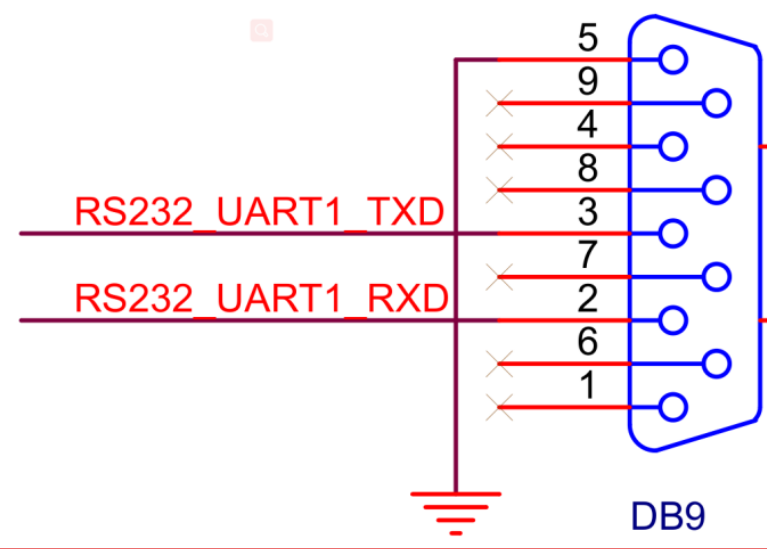
\includegraphics[width=0.5\linewidth]{figures/RS232}
	\caption{RS232}
	\label{fig:rs232}
\end{figure}

RS232 标准的接口,在电压处于-15V~-3V 时处于逻辑 1 状,当电压在+3V~+15V 时,处于逻辑 0 状态。另外在信号线这块 RTS/CTS 和 DTR/DSR 以及 CD/RI 这些信号线都是以前较老形式的,现在常用的信号线就是 RXD/TXD 和 GND 这 3 条,如果不连接 GND 地线的话可能会出现乱码。RS232 标准如下图所示:

\begin{figure}[H]
	\centering
	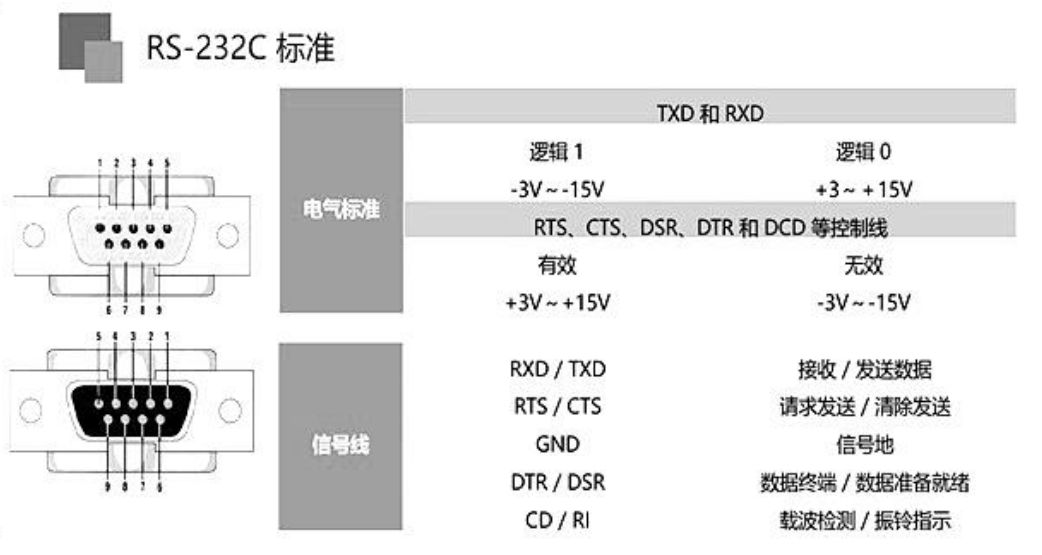
\includegraphics[width=0.7\linewidth]{figures/RS232-Stand}
	\caption{RS232标准}
	\label{fig:rs232-stand}
\end{figure}

\section{实验步骤}


程序通过/dev/ttyS3 设备节点控制串口设备节点,通过初始化波特率,模式,数据
位,停止位,流控等初始化串口。通过读写设备文件描述符来进行串口读写。

初始化串口接口函数,这里需要注意的是要把串口通信模式调成RAW模式。
\begin{minted}[breaklines=true,frame=lines]{c}
int serial_init(int *fd, const char *device) {
    struct termios Opt;
    *fd = open(device, O_RDWR | O_NOCTTY | O_NONBLOCK);
    if (*fd < 0) {
        perror("init");
        return 0;
    }
    tcgetattr(*fd, &Opt);
    cfsetispeed(&Opt, B115200);
    cfsetospeed(&Opt, B115200);
    Opt.c_iflag &= ~(IGNBRK | BRKINT | PARMRK | ISTRIP | INLCR | IGNCR | ICRNL | IXON);
    Opt.c_oflag &= ~OPOST;
    Opt.c_lflag &= ~(ECHO | ECHONL | ICANON | ISIG | IEXTEN);
    Opt.c_cflag &= ~(CSIZE | PARENB);
    Opt.c_cflag |= CS8;
    tcsetattr(*fd, TCSANOW, &Opt);

    return 1;
}
\end{minted}

串口读写接口函数:

\begin{minted}[breaklines=true,frame=lines]{c}
int serial_write(const int *fd, const char *data, size_t size) {
    int ret = write(*fd, data, size);
    if (ret < 0) {
        perror("write");
        tcflush(*fd, TCOFLUSH);
    }
    return ret;
}

int serial_read(const int *fd, char *data, size_t size) {
    ssize_t read_size = 0;
    size_t read_left = size;

    while (read_left > 0) {
        if ((read_size = read(*fd, data, read_left)) < 0) {
            if (read_size == -1)continue;
            else perror("read");
        } else if (read_size == 0) {
            break; /* EOF */
        }
        read_left -= read_size;
        data += read_size;
        printf("%s\n", data);
    }
    return (size - read_left); /* return >= 0 */
}
\end{minted}

相关逻辑:

\begin{minted}[breaklines=true,frame=lines]{c}
int main() {
    int fd = 0;
    int times = 8;
    char buf_data = rand() % 26 + 65;
    char read_buf[BUF_SIZE + 1], write_buf[BUF_SIZE];
    int ret = serial_init(&fd, dev);
    if (!ret) {
        printf("Serial Port Init Failed!!!\n");
        return -1;
    }
    printf("Start Test!!!\n");


    while (times--) {
        buf_data = rand() % 26 + 65;
        memset(write_buf, buf_data, BUF_SIZE);
        memset(read_buf, 0, BUF_SIZE + 1);

        ret = serial_write(&fd, write_buf, BUF_SIZE);
        printf("send size: %d\n", ret);

        usleep(115200 * 2);     // 保证写完

        ret = serial_read(&fd, read_buf, BUF_SIZE);
        printf("recv size: %d\n", ret);

        printf("RECV:\n%s\n", read_buf);

        ret = memcmp(read_buf, write_buf, BUF_SIZE);
        if (ret != 0) {
            printf("Result: Inconsistent data\n\n");
            break;
        } else {
            printf("Result: Consistent data\n\n");
        }

        usleep(100 * 1000);
    }
    close(fd);
    return 0;
}
\end{minted}

\paragraph{硬件连接}连接 UART0 和 PC,将网线接入 TL4379-EVM 的 RGMII ETH1 CON19 接口并接到路由器或 PC。连接好电源线,插入 SD 系统启动卡,拨码开关选择 SD 卡启动模式 00110。同时使用杜邦线将 RS232 串口的 RX 和 TX 引脚对接

\paragraph{串口连接}打开串口调试终端,选择正确的 COM 口,波特率为 115200,8N1,无检验位。

\paragraph{执行程序}开发板上电,进入开发板的操作系统,执行串口回环程序。

\section{实验总结}

通过这次实验,我实现数据的回环读写测试和校验,了解了LINUX串口通信的一般模式,了解了RS232串口,对嵌入式编程有了更深入的了解。 

\end{document}